\documentclass{article}

% Language setting
% Replace `english' with e.g. `spanish' to change the document language
\usepackage[english]{babel}

% Set page size and margins
% Replace `letterpaper' with`a4paper' for UK/EU standard size
\usepackage[letterpaper,top=2cm,bottom=2cm,left=3cm,right=3cm,marginparwidth=1.75cm]{geometry}

% Useful packages
\usepackage{amsmath}
\usepackage{graphicx}
\usepackage[colorlinks=true, allcolors=blue]{hyperref}
\usepackage{natbib}
\usepackage{amsmath,amssymb}

\title{Relazione Esercizio Timed Automata}
\author{Ruben Castelluccio}

\begin{document}
\maketitle

\section{Introduzione}
L'esercizio consiste nell'analisi mediante Timed Automata del protocollo Stop \& Wait e la sua variante per canali rumorosi. Si chiede di modellare i protocolli e di verificare le proprietà e pertanto il corretto funzionamento dei protocolli utilizzando le proprietà in TCTL.
\\Per ogni modello si identificano le seguenti entità:
\begin{itemize}
\item Mittente: per ogni messaggio inviato rimane in attesa di un Acknowledge per trasmettere un altro messaggio,
\item Destinatario: in attesa del messaggio inviato dal mittente, alla ricezione elaborarlo e trasmettere l'Acknowledge,
\item Link: canale bidirezionale e half-duplex che sincronizza il Mittente e il Destinatario.
\end{itemize}
Mittente, Destinatario e Link si sincronizza attraverso i seguenti canali:
\begin{itemize}
    \item Canale ML: sincronizzazione tra il mittente e il link
    \item Canale LM: sincronizzazione tra il link e il mittente
    \item Canale DL: sincronizzazione tra il destinatario e il link
    \item Canale LD: sincronizzazione tra il link e il destinatario
	\end{itemize}
Per lo svolgimento dell'esercizio, inoltre, sono richiesti parametri per la definizione di clock e tempo:
\begin{itemize}
    \item TT: tempo di trasmissione del messaggio lato mittente
    \item TE: tempo di elaborazione del messaggio lato destinatario
    \item TE\_min: constante intera per la definizione del valore minimo del tempo di trasmissione sull'intero sistema
    \item TE\_min: constante intera per la definizione del valore minimo del tempo di elaborazione lato destinatario
    \item TE\_max : constante intera per la definizione del valore massimo del tempo di elaborazione lato destinatario
    \item time\_min: constante intera per la definizione del valore minimo del tempo di trasmissione sull'intero sistema
    \item time\_max: constante intera per la definizione del valore minimo del tempo di trasmissione sull'intero sistema
    \item timer: constante intera per la definizione del valore con cui eseguire una ritrasmissione del messaggio pari all'incremento di uno rispetto il valore di \textit{time\_max}
    \item ACK: variabile intera definita per valore 0 o 1, utilizzata per determinare se l'Acknowledge precedente è stato perso
    \item frame\_to\_send: variabile intera definita per valore 0 o 1 per determinare il numero di seuqneza del messaggio da inviare 
\end{itemize}
\clearpage
\section{Modello A}
In questo Modello il canale è perfetto pertanto privo di perdite sia del messaggio inviato dal Mittente sia dall'Acknowledge inviato dal Destinatario. Il clock \textit{time} è utilizzato affinche il tempo di trasmissione non superi il valore massimo \textit{time max} (12) e sia superiore al valore minimo \textit{time min} (10).

\subsection{Mittente}
Il Mittente invia un messaggio e rimane in attesa di ricevere un Acknowledge dal Destinatario per poi inviare nuovamente un altro messaggio. 
\\Per l'invio del messaggio il mittente si sincronizza con il link (ML) e inizializza il clock \textit{time} a 0. Quando il link si sincronizzerà con il Mittente (LM), e pertanto avrà ricevuto l'Acknowledge potrà inviare un nuovo messaggio.
\begin{figure}[h] 
\centering
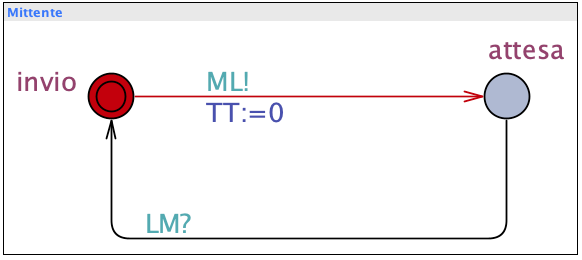
\includegraphics[scale=0.5]{modelloAM.png}
\end{figure}
\subsection{Destinatario}
Il Destinatario è in attesa della sincronizzazione con il link (LD) per la ricezione del messaggio e inizializza il clock locale \textit{ET}, procedendo all'invio dell'Acknowledge sincronizzandosi nuovamente con il link (DL) e non dovendo superare il massimo valore del clock \textit{ET\_max} definito mediante linvariante di locazione e superiore al \textit{ET\_min}, definita con la guardia.
\begin{figure}[h] 
\centering
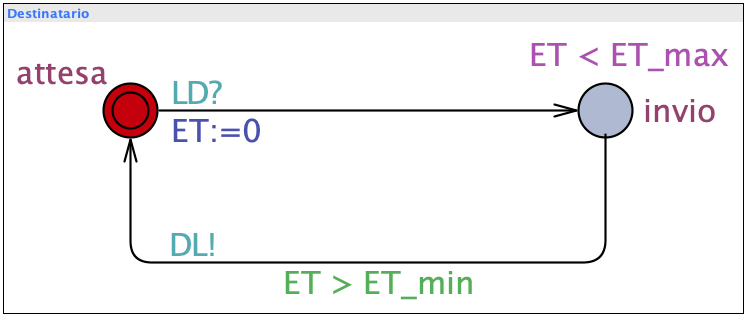
\includegraphics[scale=0.4]{modelloAD.png}
\end{figure}
\subsection{Link}
Il Link è bidirezionale, dato che il messaggio deve poter essere inviato dal Mittente e ricevuto dal Destinatario e viceversa, e allo stesso tempo half duplex pertanto il link non potrà essere utilizzato in entrambe le direzioni nello stesso momento.
\\Come speficato precedentemente viene utilizzato il clock \textit{time}, sia nella trasmissione del messaggio da Mittente a Destinatario che per l'Acknowledge da Destinatario a Mittente, definito come tempo di trasmissione del messaggio e vincolato da un limite superiore \textit{time\_max} e da un limite inferiore \textit{time\_min}. In maniera analoga a quanto avviene nel Mittente vi è la sincronizzazione (ML e LM) e allo stesso modo per il Destinatario (LD e DL).
\begin{figure}[h] 
\centering
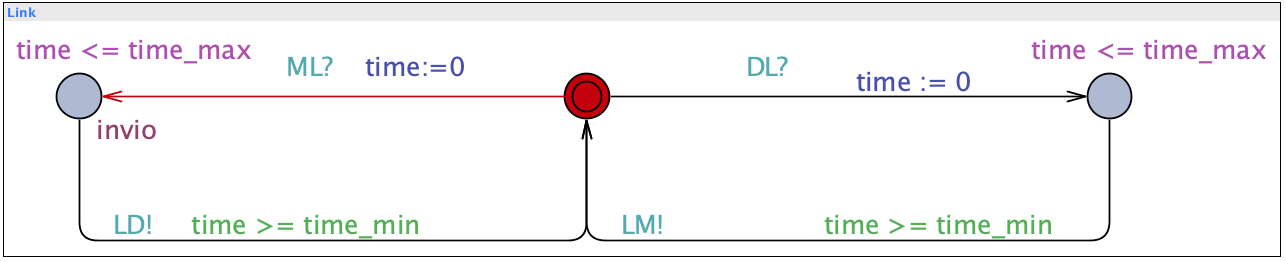
\includegraphics[scale=0.35]{modelloAL.png}
\end{figure}
\subsection{Proprietà}
\begin{enumerate}
\item Assenza di deadlock per verificare che il link sia perfetto
\begin{equation}
    A[ ] !deadlock 
\end{equation}
\item  Verifica che il Mittente dopo aver inviato il messaggio si metta in attesa dell'Acknowledge del Destinatario
\begin{equation}
Destinatario.invio --> Mittente.attesa 
\end{equation}
\item  Condizione che verifica che il Mittente ricevi tutti gli Acknowledge inviati dal Destinatario avendo un link perfetto 
\begin{equation}
Destinatario.invio --> Mittente.invio 
\end{equation}
\item Il Mittente invia il messaggio e si mette in attesa per un tempo compreso tra \textit{time\_min} e \textit{time\_max}
\begin{equation}
Mittente.attesa --> (time >= time\_min  \&\& time <= time\_max)
\end{equation}
\item Verifica che il tempo di elaborazione del messaggio da parte del destinatario sia un intervallo di tempo compreso tra \textit{ET\_min} e \textit{ET\_max}
\begin{equation}
    Destinatario.ET == 0 \&\& Destinatario.attesa --> 
    \end{equation}
    \begin{equation}
        (Destinatario.ET >= 
    Destinatario.ET\_min \&\& Destinatario.ET <= Destinatario.ET\_max)
 \end{equation}
 \item Il tempo di trasmissione del messaggio sul link è compreso tra \textit{timemin} e \textit{timemax}
\begin{equation}
    time == 0 \&\& Link.invio --> (time >= time\_min \&\& time <= time\_max)
\end{equation}
\end{enumerate}
\clearpage
\section{Modello B}
Il modello B si differenzia dal modello A in quanto presenta la possibilità che sia il messaggio sia l' Acknowledge possano esser persi nella comunicazione pertanto il link non è più perfetto mentre la struttura del mittente e destinatario rimane inalterata.

\subsection{Link}
Il Link presenta la stessa struttura del modello A ad eccezzione dell'aggiunta di un arco sia per il mittente sia per il destinatario in modo da non sincronizzarsi con le altre entità simulando la perdita del messaggio dell'Acknowledge.
\begin{figure}[h] 
\centering
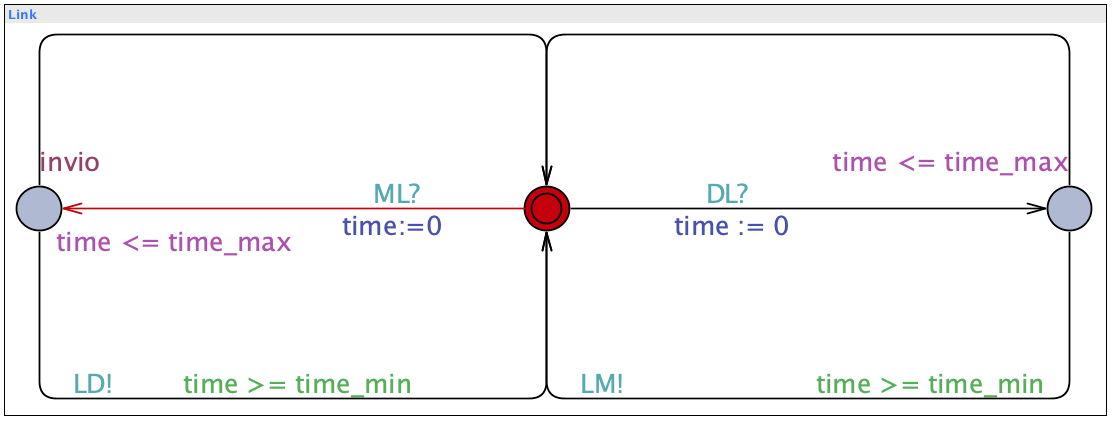
\includegraphics[scale=0.4]{modelloBL.png}
\end{figure}
\subsection{Proprietà}
\begin{enumerate}
    \item Assenza di deadlock non verificata in quanto nella struttura del Link è possibile che non avvenga la sincronizzazione sia lato mittente sia lato destinatario.
    \begin{equation}
    A[ ] !deadlock 
    \end{equation}
\item Non è verificata la condizione per cui il Mittente dopo aver inviato il messaggio si metta in attesa dell'Acknowledge del Destinatario in quanto il canale è soggetto a perdite di messaggi pertanto il Destinatario non si sincronizzerà con il link in quanto il messaggio è stato perso.
\begin{equation}
Mittente.attesa \&\& time == 0 --> Destinatario.invio
\end{equation}
\item Non è verificata la condizione per cui il tempo di trasmissione è limitato nell'intervallo tra \textit{time min} e \textit{time max} mentre il Mittente è in attesa della ricezione dell'Acknowledge da parte del Destinatario
\begin{equation}
    Mittente.attesa --> (time >= time\_min  \&\& time <= time\_max)
\end{equation}
\item  Condizione non verificata per cui il Mittente non riceva gli Acknowledge inviati dal Destinatario avendo un link con perdita
\begin{equation}
Destinatario.invio --> Mittente.invio 
\end{equation}
 \item Il tempo di trasmissione del messaggio sul link è compreso tra \textit{time\_min} e \textit{time\_max}
\begin{equation}
    time == 0 \&\& Link.invio --> (time >= time\_min \&\& time <= time\_max)
\end{equation}
    
\end{enumerate}
\clearpage
\section{Modello C}
Nel modello C si richiede di mantenere il comportamento del link analogo al modello B, pertanto un canale con perdita di messaggio o di Acknowledge, ma modificando il mittente e destinatario al fine di risolvere le problematiche presenti nel modello B in cui a seguito di una perdita non vi era ritrasmissione. 
\\ Pertanto in questo modello viene aggiunto un timer che allo scadere farà eseguire una ritrasmissione del messaggio  verificando la corrispondenza tra il numero di sequenza del messaggio inviato dal mittente e l'Acknowledge inviato dal destinatario. 
\subsection{Mittente}
Alla struttura del mittente, rispetto al modello A e modello B, viene aggiunto un timer nella locazione di attesa dell'Acknowledge e se viene superato il limite superiore \textit{time\_max} il messaggio sarà andato perduto perciò viene definita una nuova locazione \textit{ritrasmissione}, pertanto avviene nuovamente la sincronizzazione con il link e viene ri-inizializzato il tempo di ritrasmissione \textit{time}.
\begin{figure}[h] 
\centering
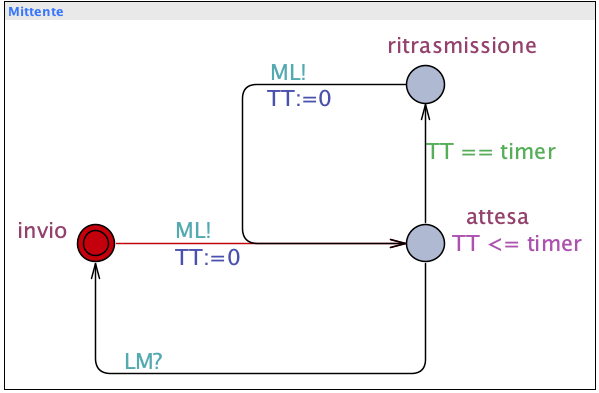
\includegraphics[scale=0.4]{modelloCM.png}
\end{figure}
\subsection{Destinatario}
Analogamente a quanto avviene nel caso del mittente anche nel destinatario vi è l'aggiunta di un arco, che come nel modello A e nel modello B, si sincronizza con il link ma differenziato dalla guardia che richiede di verificare se il numero dell' \textit{ACK} e del numero del messaggio sono differenti, inoltre viene aggiunta un ulteriore guardia sull'arco gia presente in cui si verifica se l'\textit{ACK} ha lo stesso numero della sequenza del messaggio.
\begin{figure}[h] 
\centering
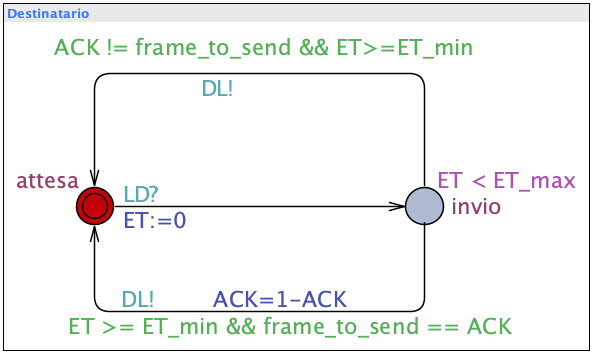
\includegraphics[scale=0.5]{modelloCD.png}
\end{figure}
\subsection{Proprietà}
\begin{enumerate}
    \item Assenza di deadlock verificata in quanto il mittente e destinatario, nel caso di avvenuta perdita, permetteno la ritrasmissione.
    \begin{equation}
    A[ ] !deadlock
    \end{equation}
\item  Condizione non verificata in quanto il link prevede la perdita del messaggio o dell'Acknowledge per cui vi è la possibilità che il Destinatario debba ritrasmettere l'Acknowledge 
\begin{equation}
Destinatario.invio --> Mittente.invio 
\end{equation}
 \item Verifico che il tempo di trasmissione del messaggio sul link è compreso tra \textit{time\_min} e \textit{time\_max}
\begin{equation}
    time == 0 \&\& Link.invio --> (time >= time\_min \&\& time <= time\_max)
\end{equation}
\item Condizione non verificata in quanto il Mittente invia il messaggio e si mette in attesa per un tempo che non è compreso nell'intervallo di tempo tra \textit{time\_min} e \textit{time\_max} dato che il link prevede la perdita dell'Acknowledge 
\begin{equation}
Mittente.attesa --> (time >= time\_min  \&\& time <= time\_max)
\end{equation}
\item Verifica che il tempo di elaborazione del messaggio da parte del destinatario sia un intervallo di tempo compreso tra \textit{ET\_min} e \textit{ET\_max}
\begin{equation}
    Destinatario.ET == 0 \&\& Destinatario.attesa --> 
    \end{equation}
    \begin{equation}
        (Destinatario.ET >= 
    Destinatario.ET\_min \&\& Destinatario.ET <= Destinatario.ET\_max)
 \end{equation}
\end{enumerate}
\clearpage
\section{Considerazioni Finali}
D: E' possibile identificare un valore di timer che ci permette di affermare con certezza se il timer scatta il messaggio è stato perso? Questo valore che ha impatto ha sull'efficienza del canale trasmissivo?
\\R: Il valore che viene attribuito al timer è determinante per l'efficienza del canale trasmissivo in quanto determina con certezza l'avvenuta perdita del messaggio e la conseguente ritrasmissione. Potendo lavorare solo su interi il primo valore possibile è l'incremento di unità rispetto al massimo valore del tempo di trasmissione.
\\\\
D:L'algoritmo prevede l'utilizzo di 2 timer, uno per ogni possibile numerazione dei messaggi: sono davvero necessari ambedue?
\\R:E' sufficiente l'impiego di un solo timer data la natura half duplex del link che non permette nello stesso momento l'attraversamento sia di un messaggio sia di un Acknowledge.
\end{document}
